\documentclass[UKenglish]{uiomasterthesis}
\usepackage[utf8]{inputenc}                
\usepackage[T1]{url}\urlstyle{sf}
\usepackage{babel, csquotes, graphicx, textcomp, uiomasterfp, varioref}
\usepackage[backend=biber,style=numeric-comp]{biblatex}
\usepackage[hidelinks, hypertexnames=false]{hyperref}
\usepackage{url}
\usepackage{verbatim}
\usepackage{amsmath,amssymb,amsfonts}
\usepackage{hyperref}
\usepackage{cleveref}
\usepackage{algorithmic}
\usepackage{graphicx}
\usepackage{textcomp}
\usepackage{xcolor}
\usepackage{caption} 
\usepackage{nicefrac}
\usepackage{float}
\usepackage{multirow}
\usepackage{tabularx}
\usepackage{booktabs}

\addbibresource{project.bib}

\author{Tonje Viddal Sandanger}
\title{Enhancing Gait Analysis through eXplainable AI}
\begin{document}
\uiomasterfp[
    master, 
    program={Informatics: Robotics and Intelligent Systems},
    color=blue, dept={Department of Informatics}, 
    fac={Faculty of Mathematics and Natural Sciences},
    supervisors={Professor Jim Tørressen \and Dr. Ola Wiig \and Eirik Gromholt Homlong \and Rahul Prasanna Kumar},
    long
]                                

\frontmatter{}
\begin{abstract}
  Here come 3--6 sentences describing your thesis.
\end{abstract}

\begin{xabstract}[Sammendrag]               
  Here comes the abstract in a different language.
\end{xabstract}

\tableofcontents{}                          
\listoffigures{}                            
\listoftables{}                             

\begin{preface}
  Here comes your preface, including acknowledgments and thanks.
\end{preface}

\mainmatter{}
\part{Introduction}                   
\chapter{Background}                 
\section{Classification and Clinical Use Case}
In the management of Cerebral Palsy (CP), classifying gait patterns is key to diagnosing severity and guiding treatment. This section explores the gait abnormalities characteristic of CP. Understanding these patterns is not only critical for patient care but also informs the long-term treatment efficacy and provides a framework for ongoing research in CP therapies.

\subsection{Gait Patterns in Cerebral Palsy}
The gait patterns used to classify CP, as seen in Fig.~\ref{fig:Gait Pattern}, can be summarized as \cite{papageorgiou_systematic_2019}: 

\begin{itemize}
    \item{\textbf{Genu Recurvatum:} Characterized by hyperextension of the knee, which may be accompanied by either plantarflexion or reduced dorsiflexion at the ankle. This pattern is often observed when the knee extends beyond its normal range during the stance phase, sometimes leading to an unstable or backward-bending knee appearance.}
    
    \item{\textbf{Drop Foot:} This pattern is defined by a weakness or paralysis of the muscles that lift the foot, resulting in a downward-pointing foot during the swing phase. It often leads to a compensatory high stepping gait to prevent the toes from dragging on the ground.}
    
    \item{\textbf{True Equinus:} The ankle remains in plantarflexion throughout the stance phase, with the hips and knees fully extended. This gait pattern often results in a toe-walking appearance due to the ankle's plantarflexed position.}
    
    \item{\textbf{Jump Gait:} Characterized by equinus at the ankle along with flexion at the knee and hip. This pattern also includes an anterior pelvic tilt and an exaggerated lumbar lordosis, leading to a distinctive gait where the knees and hips are bent while the ankles are plantarflexed.}
    
    \item{\textbf{Apparent Equinus:} Although the ankle demonstrates a normal range of dorsiflexion, excessive flexion at the hip and knee throughout the stance phase gives the appearance of walking on the toes. This creates the impression of equinus, despite the ankle being in a neutral or dorsiflexed position.}
    
    \item{\textbf{Crouch Gait:} Marked by excessive dorsiflexion at the ankle, coupled with significant flexion at the knee and hip joints. This pattern results in a crouched posture during walking, where the knees and hips are bent more than usual, leading to a lower center of gravity.}
    
\end{itemize}


\begin{figure}[ht]
    \centering
    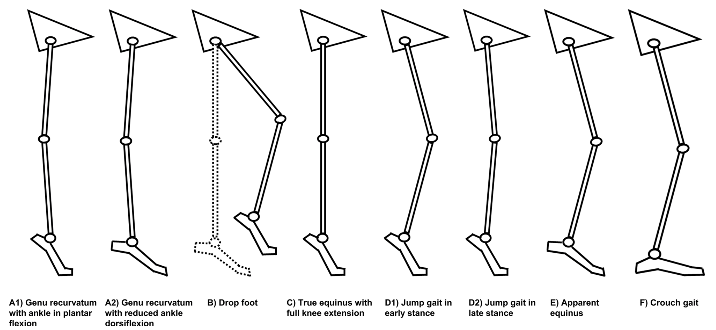
\includegraphics[width=1\linewidth]{Figures/GaitImage.png}
    \caption{This figure, as seen in \cite{papageorgiou_systematic_2019}, illustrates six types of gait abnormalities: A1) Genu Recurvatum with ankle in plantar flexion, A2) Genu Recurvatum with reduced ankle dorsiflexion, B) Drop Foot, C) True Equinus with full knee extension, D1) Jump Gait in early stance, D2) Jump Gait in late stance, E) Apparent Equinus, and F) Crouch Gait. Each diagram represents the characteristic joint positions and angles associated with these specific gait patterns.}
    \label{fig:Gait Pattern}
\end{figure}

\subsection{Clinical Application of Gait Analysis}

There are multiple use-case areas of the clinical application of these classifications. Precise identification of gait abnormalities would allows clinicians to:

\begin{itemize}
    \item Develop customized rehabilitation plans that address the unique motor challenges encountered by each patient.
    \item Prescribe appropriate orthotic devices to improve ambulatory ability and independence.
    \item Monitor the progression of CP and the effectiveness of interventions over time.
    \item Inform surgical decision-making processes, such as determining the necessity and nature of orthopedic surgery.
    \item Aid in predicting future mobility issues and proactively manage potential complications.
\end{itemize}

Furthermore, classifying gait patterns extends beyond immediate clinical interventions. By providing a solid quantitative basis for long-term research, classifying gait patterns would expand our knowledge of how CP evolves over time and how different treatments can affect patient outcomes in the long run. By utilizing machine learning, clinicians have the potential to match gait pattern data with clinical outcomes, refining treatment protocols and enhancing predictive analytics in patient care. The integration of gait classification tools within a clinical setting showcases a promising combination of technology and medicine.

\section{Machine-Learning Models}
When choosing a classification method, various machine learning (ML) methods was considered. Given the three-dimensional nature of the dataset, it's important to choose models that exhibit sufficient performance with such handling such data structures. Employing 3D Convolutional Neural Networks (3D-CNNs), as well as decision trees or random forests is an interesting area to explore, particularly as the literature hasn't yeat explored these topics so extensively.

Selecting CNNs was partly done as Slijepcevic et al. has performed a classification of a similar purpose only with a two-dimensional CNN having moderate success \cite{slijepcevic_explainable_2023}. By extending this investigation to encompass three-dimensional data points, the present study aims to address certain gaps within the existing literature, thereby contributing to a more comprehensive understanding of the classification task.
Furthermore, the selection of random forests and decision trees aligns with their demonstrated efficacy in similar experiments. Given their robust performance in CP classification tasks, testing their performance on 3D points could be an interesting angle for investigation. 

\subsection{Three-dimensional Convolutional Neural Network}
A three-dimensional Convolusional Neural Network (3D CNN) is a neural network architecture consisting of multiple layers that can learn abstract feature representations for three dimensional data. These feature representations can be used for tasks such as classification, generation, or regression. These models are programmed to analyse data with spatial and temporal dimensions, and are also able to process sensor data like point clouds. This is achieved through developing models with multiple channels which captures information from input frames as done by Ji et al. \cite{ji_3d_2013}.  

The use of classification with 3D CNNs would be combined with Grad-CAM. 

\subsection{Decision Trees and Random Forests}
In addition to employing 3D CNNs, an interesting angle of investigation could be to explore the use of Decision Trees (DT) and Random Forests (RF). Tree based models are popular for gait-classification for their non-linear, and non-parametric properties as well as their simplicity \cite{figueiredo_automatic_2018}. Initially introduced by Belson \cite{belson_matching_1959}, a decision tree is a classification model that operates via a recursive partitioning of the instance space \cite{maimon_decision_2005}. This tree structure consists of nodes connected by edges, with each node having precisely one incoming edge. Nodes with solely an incoming edge are called a leaf node. Some nodes features an outgoing edge , and are referred to as internal nodes, responsible for dividing the space into two homogeneous sub-spaces. It's common to employ a metric, impurity, to decide which feature fits into which decision node. The features importance is therefore decided by how much it contributes to reducing the total impurity of the tree. 

Decision trees have a tendency to be highly sensitive to small changes in the input data, therefore making the decision to deploy RF could combat this. A RF is made by training a predetermined number of decision trees, and then combining the predictions of these trees. RF are sensitive to the number of trees and a grid search will therefore be performed to ensure the best performance. 

For this experiment, the implementation of decision trees would be combined with the use of SHAPley values.

\subsection{Recurrent Neural Network}
Recurrent Neural Networks (RNNs), proposed by Rumelhart et al. \cite{rumelhart_learning_1986}, are a class of neural networks that are designed to handle sequential data \cite{goodfellow_deep_2016}. Unlike traditional feedforward neural networks, which assume that inputs are independent of each other, RNNs are built to recognize the sequential nature of data and can use their internal state (memory) to process sequences of inputs. This makes them particularly well-suited for tasks like language modeling, speech recognition, and time series prediction.

The fundamental idea behind RNNs is to have neurons that activate in a loop, allowing information to persist and be passed along the sequence of inputs. In the traditional formulation, at each timestep of processing, an RNN takes two pieces of information: the current input vector and the hidden state from the previous timestep. The hidden state acts as the memory of the network that captures information about what has been processed so far.

\begin{figure}
    \centering
    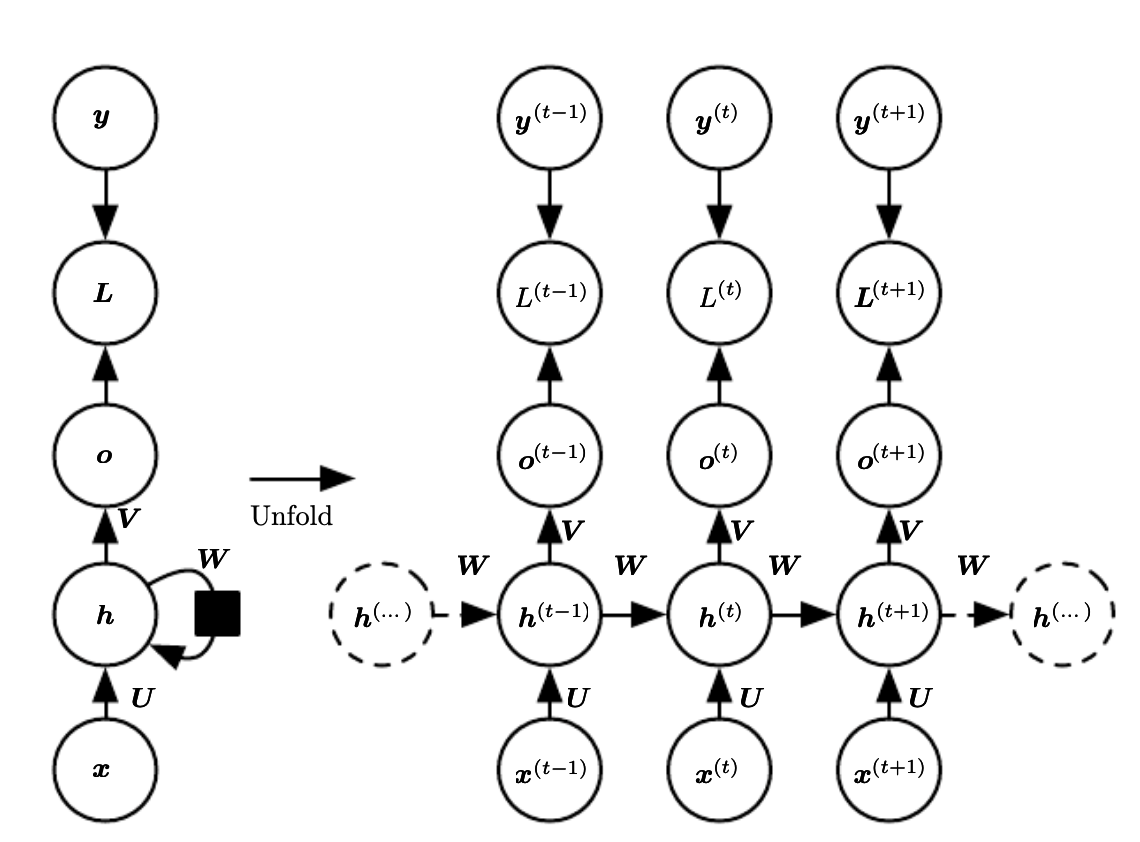
\includegraphics[width=0.7\linewidth]{Figures/RNN.png}
    \caption{A RNN where it takes input values (x) and produces output values (o). The loss (L) measures how different each output (o) is from the expected target (y). When using softmax outputs, we treat o as unnormalized log probabilities. The loss internally computes \begin{math}\hat{y}\end{math} by applying softmax to o and compares it to the target y. The RNN has connections from input to hidden (U), hidden to hidden (W), and hidden to output (V). The graph can be visualized with recurrent connections (Left) or as a time-unfolded graph where each node represents a specific time instance (Right) \cite{goodfellow_deep_2016}.}
    \label{fig:RNN}
\end{figure}

RNNs can be trained using the backpropagation algorithm, like any other neural network, however, for sequences, the process is called backpropagation through time (BPTT). BPTT unrolls the RNN through time and applies the backpropagation algorithm to compute gradients and update weights, considering the entire input sequence \cite{goodfellow_deep_2016}.

\subsection{Transformers}
The Transformer is a powerful neural network architecture, as seen in Fig: \ref{fig:Transformer}, revolutionizing natural language processing. It utilizes self-attention mechanisms, enabling it to capture dependencies across input sequences efficiently. Introduced in the paper "Attention is All You Need" by Vaswani et al. \cite{vaswani_attention_2023}, the transformer has an encoder-decoder structure, which processes input tokens into contextualized representations and generates output sequences. Multi-head attention allows parallelized processing of different aspects of the input, while positional encodings maintain sequence order information. Through these innovations, the Transformer has achieved state-of-the-art performance in various language tasks, marking a significant advancement in the field.

\textbf{Encoder-Decoder} The encoder consists of 6 identical layers, each comprising two sub-layers: a multi-head self-attention mechanism and a position-wise fully connected feed-forward network. Residual connections and layer normalization are applied around each sub-layer, producing outputs of dimension dmodel = 512.


\textbf{Attention} is a mechanism used in neural networks to weigh the importance of different elements in a set, often referred to as the key-value set, with respect to the query. Each element in the key-value set is associated with both a key and a value.

The attention mechanism computes the output by applying a softmax function to the compatibility scores between the query and each key in the key-value set, resulting in weights that determine a weighted sum of the values. This allows the model to focus more on relevant elements of the key-value set when producing the output based on the given query. 

\textbf{Scaled Dot-Product Attention}, as seen in Fig: \ref{fig:mha} (left), has queries (Q), keys (K) and values (V) as inputs. The dot products of the queries with keys are computed, scaled, and then softmaxed, to derive weights on the values (V). This is then applied to sets of queries, keys, and values simultaneously, arranged in matrices Q, K, and V respectively. 

There are two commonly used attention functions: additive attention and dot-product attention. Dot-product attention, as described, is faster and more space-efficient due to optimized matrix multiplication. However, for larger values of d, additive attention outperforms dot product attention without scaling. We use scaling to mitigate issues with large dot products.

\textbf{Multi-Head Attention}, as seen in Fig: \ref{fig:mha} (right), enables the model to collectively attend to information from various representation subspaces at different positions. Instead of utilizing a single attention function with keys, values, and queries of dmodel dimensions, Vaswani et al. opt to linearly project them h times using different learned linear projections the inputs respective dimentions. This allows for parallel attention computations on each projected version, resulting in dv-dimensional output values. These outputs are then concatenated and projected again to obtain the final values. To make the computational cost, a reduction of dimensions is performed.

\begin{figure}
    \centering
    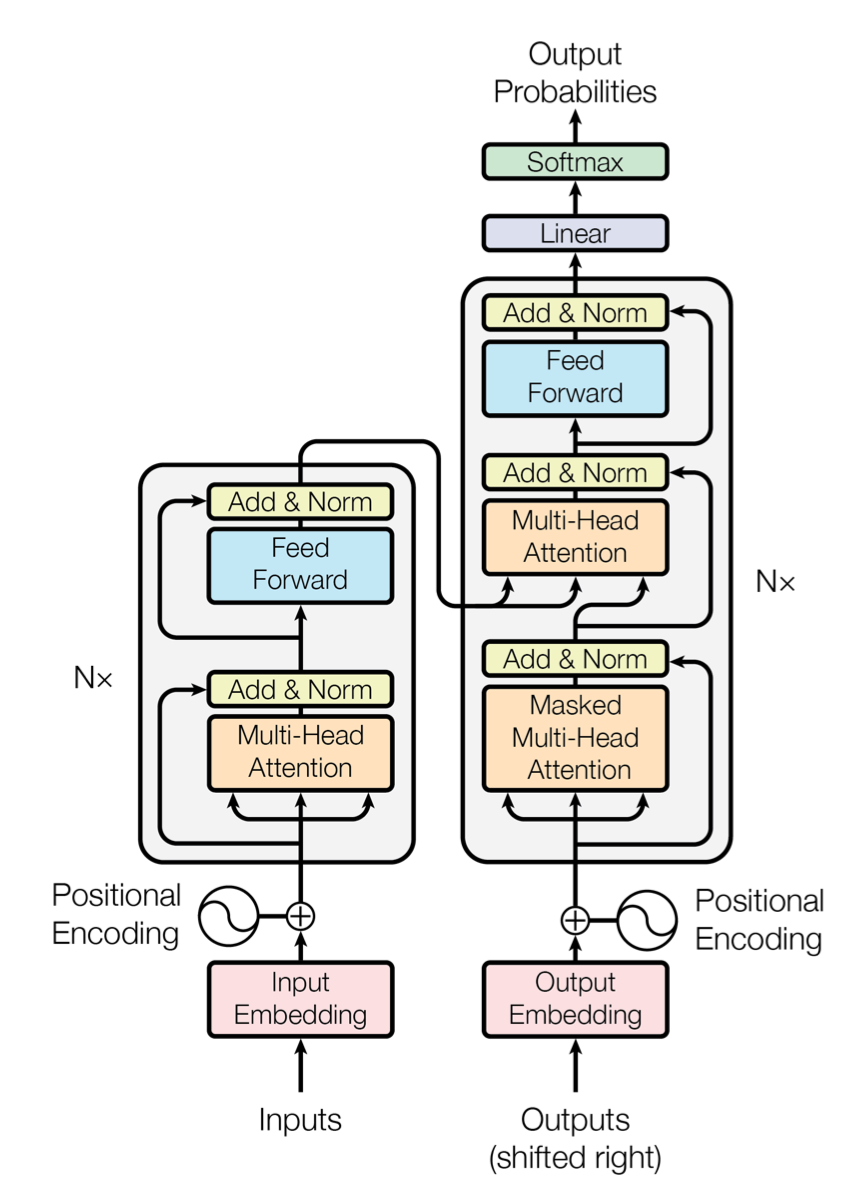
\includegraphics[width=0.65\linewidth]{Figures/transformer.png}
    \caption{Model Architecture of a Transformer as seen in Vaswani et al \cite{vaswani_attention_2023}.}
    \label{fig:Transformer}
\end{figure}

\begin{figure}
    \centering
    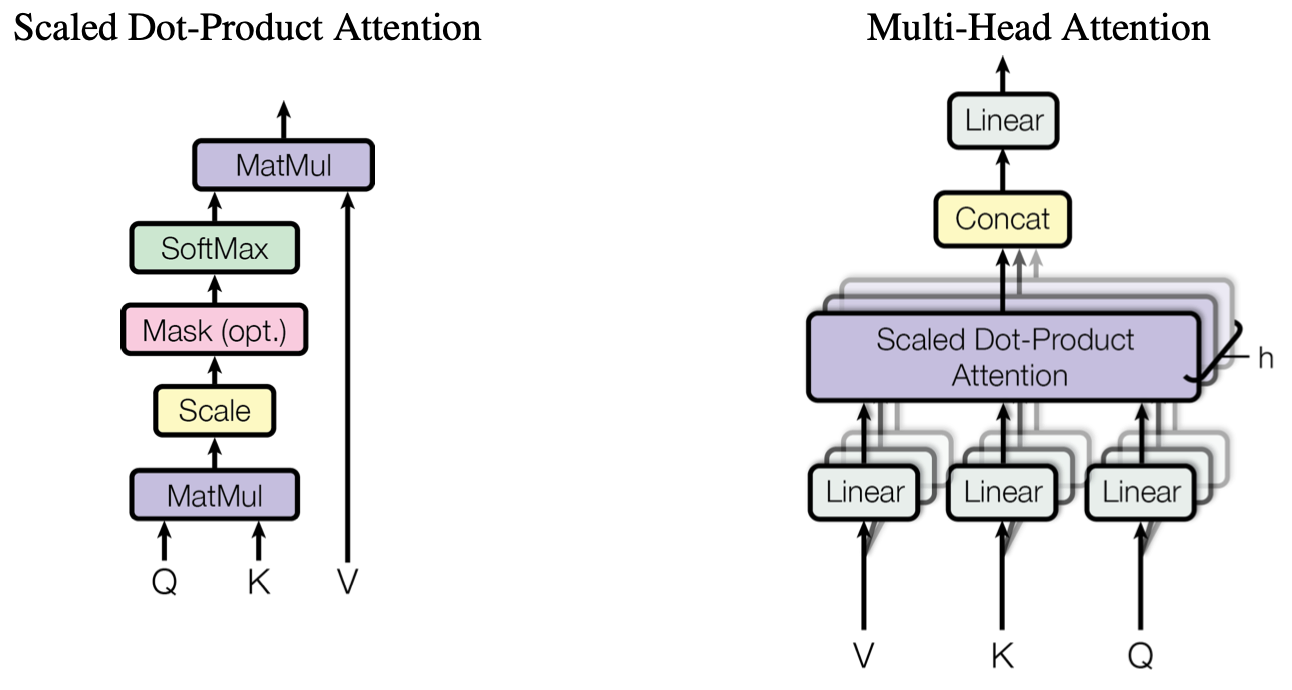
\includegraphics[width=0.85\linewidth]{Figures/mha.png}
    \caption{Scaled Dot-Product Attention (left) and Multi-Head Attention (right) as seen in Vaswani et al \cite{vaswani_attention_2023}.}
    \label{fig:mha}
\end{figure}

\section{eXplainable Artificial Intelligence}

\subsection{Model Agnostic}
In machine learning, when referring to model agnostic methods, we refer to methodologies and techniques that are independent of the specific model employed. These approaches aim to provide generalized solutions applicable across diverse machine learning algorithms, irrespective of their underlying architectures or characteristics.

Examples of techniques which employs such feature importance analysis methods, is SHAP and LIME. These methodologies can be seamlessly applied to various machine learning models, including decision trees, neural networks, support vector machines, and others, without necessitating modifications specific to each model.

\subsubsection{SHapley Additive exPlanations}
SHAP (SHapley Additive exPlanations) is a framework for interpreting model predictions. \cite{lundberg_unified_2017} The method is motivated by the increasing need for accurate and interpretable explanations in machine learning models, especially in the world of complex models like ensamble methods and deep learning networks. It addresses the challenges of understanding the complex models by assigning them importance values to each feature for a given prediction. 

The framework unifies six existing methods under the class of additive feature attribution methods, which ensures properties like local accuracy, missingness, and consistency. These properties are crucial for maintaining the interpretability and reliability of the explanations provided. SHAP values emerge as a unique measure of feature importance that satisfies these properties and utilizes conditional expectations to define simplified inputs. 

The paper presents various approximation methods for computing SHAP values, both model-agnostic and model-specific, each tailored to different types of models. Experimental results demonstrate the superiority of SHAP values over alternative methods in terms of computational efficiency and consistency with human intuition. User studies and comparisons with existing methods validate the effectiveness of SHAP in providing interpretable explanations for model predictions. Overall, SHAP offers a promising framework for bridging the gap between accuracy and interpretability in machine learning applications, with avenues for further research focused on enhancing computational efficiency and exploring interaction effects from game theory to improve interpretability further \cite{lundberg_unified_2017}.

\subsubsection{Local Interpretable Model-agnostic Explanations}
As proposed by Ribeiro et al. LIME is an model agnostic explanation technique that helps explain the predictions of any classifier or regressor by approximating it locally with an interpretable model \cite{ribeiro_why_2016}. LIME, short for Local Interpretable Model-Agnostic Explanations, offers a breakthrough method for interpreting machine learning models, particularly in cases where the inner workings of a model are opaque. It functions by generating explanations, as according to Equation \ref{eq1} where G is G is a linear models, \begin{math} \mathcal{L} \end{math}
is the loss, \begin{math} \pi_{x}\end{math} is the proximity measure between z and x and \begin{math} \Omega_{g} \end{math} is the regularization term for model complexity. 

\begin{equation}
    \label{eq1}
    \xi (x) = argmin_{{g\in G}} \text{ } \mathcal{L}(f,g,\pi_{x}) + \Omega (g)
\end{equation}

The process happens through a series of steps: 
\begin{enumerate}
    \item Samples are selected by permuting features of the test samples x. 
    \item A kernel calculation values the weights of the samples and the x.
    \item  The model g is then trained to predict f(x) that approximates the behavior of the original black-box model in the vicinity of the selected samples to feature importance estimate.
\end{enumerate} 

This interpretable model provides insights into the features driving the model's decision-making process, offering a clear view of which factors influence the predictions the most. By focusing on local approximations, LIME provides explanations that are intuitive and actionable, allowing users to understand and trust their models better. It's a versatile tool that can be applied to various types of data, including tabular, text, and image data, with adjustments made to maintain interpretability. Overall, LIME empowers users to delve into the intricacies of machine learning models, uncovering biases, identifying errors, and ultimately improving model performance and trustworthiness.

\subsection{Gradient-weighted Class Activation Mapping}
The field of computer vision and deep learning has seen a surge in research aimed at enhancing the interpretability of Convolutional Neural Networks (CNNs) through visualization techniques. Prior works have explored methods like saliency maps to highlight crucial pixels in CNN predictions, shedding light on the inner workings of neural networks. Understanding the trustworthiness and faithfulness of deep learning models has become paramount, with weakly-supervised localization techniques playing a key role in elucidating model decisions.

Gradient-weighted Class Activation Mapping (Grad-CAM), a groundbreaking approach, merges high-resolution visualizations with class-discriminative strategies to offer precise and reliable visual explanations derived from deep networks. Its versatility is evident in applications across various architectures for tasks such as image classification, image captioning, and Visual Question Answering (VQA), showcasing its broad utility and effectiveness. By providing interpretable visual explanations without the need for an explicit attention mechanism, Grad-CAM advances the comprehension of intricate model decisions, contributing to the transparency and trustworthiness of deep learning models.

In essence, the integration of Grad-CAM with existing visualization methodologies marks a significant stride towards transparent and dependable deep learning models. This advancement not only enhances interpretability but also fosters reliability in artificial intelligence and machine learning applications, paving the way for more trustworthy and understandable AI systems.

\section{Methods}

\subsection{3D Gait Data for Machine Learning}
The 3D gait analysis data was collected at Oslo University Hospital (OUS) using a Vicon motion capture system (©VICON Motion Systems Ltd, UK) \cite{noauthor_vicon_nodate}. This system employs eight infrared cameras, capturing motion at a rate of 100 frames per second. Reflective markers were strategically placed on the lower limbs, utilizing Vicon’s lower body Plug-in-Gait model, which is based on the Newington-Helen Hayes gait model \cite{kadaba_measurement_nodate}, \cite{davis_iii_gait_nodate}. After the clinical gait analysis, the data was postprocessed using the same model to calculate joint angles. During this postprocessing phase, foot contact points were manually timed, annotated, and saved as events in C3D format.

Data was collected from 63 patients, and 70 affected legs were classified into one of the six patterns described above: genu recurvatum (N = 8), drop foot (N = 13), true equinus (N = 26), jump gait (N = 11), apparent equinus (N = 7), and crouch gait (N = 5). 

The dataset encompasses details regarding joint angles (kinematics) for the pelvis, hip, knee, and ankle, as well as Ground Reaction Forces (GRFs) across all three planes of motion. Gait kinematics are described in relation to the sagittal, frontal, and transverse planes, representing flexion/extension, abduction/adduction, and internal/external rotation of joints, respectively. The analysis was carried out separately for individual legs and for both legs collectively. In the case of individual leg analysis, classifications were made and subsequently compared to the corresponding to discern whether the affected leg exhibited distinctions from the others in the same class.

Due to a partly unbalanced dataset, it´s still unsure how much data will end up being included in the official dataset. This means that the amount of data may change depending on how much data we are able to label. 

\subsection{Classification Method for time series data}

\subsubsection{XAI techniques for Recurrent neural networks}
For time series data it's possible to use an RNN as it is adapted for sequential data. 
We can utilize RNNs to interpret data by employing attention mechanisms. Attention assigns significance values to various timestamps in the data, reflecting their importance. Karim et al. has used a LSTM Fully Convolutional Network to perform time series classification \cite{karim_lstm_2018} with success. 
Choi et al. blend CNN and LSTM models for learning temporal dependencies, using LSTM states for classification with attention weights which indicates time step importance. They extend this by stacking neural network layers for variable attention \cite{choi_prediction_2019}. Vinayavekhin et al. compute focused attention across all time steps \cite{vinayavekhin_focusing_2018}, while Ge et al. derive variable attention directly from LSTM weights \cite{ge_interpretable_nodate}.
It is also possible to focus on the globally important variables, not just locally, as attention mechanisms are used in transformers \cite{vaswani_attention_2023} This would make it possible to learn the relations between different temporal scales.
Lastly, it is also possible to explain recurrent models by using model agnostic methods such as LIME \cite{ribeiro_why_2016} and SHAP \cite{lundberg_unified_2017} as mentiones previously. 

\subsubsection{XAI techniques for 3D-CNNs}
It is also possible to use CNNs to explain time series data. There are two main ways we explain using a CNN on time series data, perturbation-based methods and backpropagation-based methods. 

\textit{Backpropagation method: } This method is what is originally used to explain deep learning based image analysis, however it is possible to use it on time series data as Wang et al.\cite{wang_time_2016} and Fawaz et al.\cite{fawaz_evaluating_2018} has done. When combining a 3D-CNN with the Grad-CAM method as a post-hoc method, it gives highlighted areas of the regions that the CNN used as the most important information for classification. This method can also highlight sub-sequences of the time series data. It uses global average pooling layers to summarize channel activations, then assigns weights per filter using softmax. This creates heatmaps representing each class. Upsampling these heatmaps reveals relevant sub-sequences \cite{rojat_explainable_2021}.

\textit{Perturbation-based methods:} Perturbation-based methods calculate feature importance by altering input features and measuring the difference in model output \cite{ancona_towards_2018}. Higher differences indicate higher feature contribution. SHAP and LIME would be examples of those. 

\subsection{Performance measures}
When measuring the performance of the models, different methods were used. The models were each measured on accuracy, recall, precision, and F1 scores was computed using the true positives (TP), true negatives (TN), false positives (FP) and false negatives (FN). In Table \ref{table1} the methods and their formulas, as well as a description of the use. These measures would help us indicate whether the model was successful in the estimation of gait analysis. 

\begin{table*}[!ht]
\centering
\begin{tabularx}{\textwidth}{>{\hsize=0.5\hsize}X>{\hsize=0.9\hsize}X>{\hsize=1.7\hsize}X}
\toprule
\textbf{Measure} & \textbf{Formula} & \textbf{Description} \\
\midrule
Accuracy & \(\frac{TN+TP}{TP+TN+FP+FN}\) & How many correctly classified gait abnormalities were performed by the models. This is defined as the number of true positives and true negatives divided by all cases.\\
\midrule
Recall & \(\frac{TP}{TP+FN}\) & The ability of a model to find all the relevant cases within a data set. The number of true positives divided by the number of true positives plus the number of false negatives.\\
\midrule
Precision & \(\frac{TP}{TP+FP}\) & Precision refers to the fraction of relevant instances among the retrieved instances. It is the number of true positives divided by the number of true positives plus false positives.\\
\midrule
F1 Score & \(2 \times \frac{Precision \times Recall}{Precision + Recall}\) & The F1 Score is the harmonic mean of precision and recall, providing a balance between the two in cases where one might have much higher values than the other.\\
\bottomrule
\end{tabularx}
\caption{Performance measures, formulas, and description}
\label{table1}
\end{table*}

\newpage
\section{Ethical Concideration}
The handeling of patient data, in the context of 3D gait analysis, demands a commitment to privacy and confidentiality. Measures in this study are anonymized, in line with established legal and ethical standards set by the Norwegian Research Counsil (NRC). 

\subsection{Data Privacy and Algorithmic Transparency}

To counter potential ethical concerns that is associated with the application of artificial intelligence, the visualization tool incorporated XAI. This ensures transparency in the decision making of the algorithm, allowing for a deeper understanding of the outcomes. The visualization tool is also developed following the principle of universality, aiming for accessibility and unbiased representation of data. The tool is developed to be user friendly, regardless of individual differences.

Our ethical approach involves using a normalized and diverse dataset for training the machine learning model, ensuring fairness and reliability across various cerebral palsy gait patterns.

Lastly the algorithm itself will undergo testing and verification, ensuring a non-bias and fair algorithm. The goal is to minimize discrimination in the outcomes. This commitment extends to fostering a culture of openness, transparency, and continuous improvement in the ethical dimensions of the research.

\subsection{Navigating the Challenges of XAI in Healthcare}
Despite the promise of XAI to provide insights into the decision-making processes of machine learning models, there are several limitations and challenges that researchers and practitioners must navigate in order to integrate it into the world of healthcare. In the context of gait analysis, these limitations can impact both the performance of XAI systems and their acceptance by clinicians and patients.

One of the primary challenges in XAI is generating explanations that are both accurate and intuitive for users. There is an inherent trade-off between the fidelity of an explanation and its interpretability \cite{holzinger_causability_2019}. High-fidelity explanations that closely reflect the model's operations can be too technical, whereas more interpretable explanations may oversimplify the model's logic, potentially leading to misinterpretation or a false sense of understanding.

The field of XAI lacks a standardized framework for evaluating explanations, making it difficult to assess their quality and reliability \cite{liu_tensors_2022} Without universally accepted metrics, it is challenging to compare the effectiveness of different XAI approaches and validate their usefulness in clinical settings.

Implementing XAI in healthcare settings often involves processing sensitive patient data. Since some XAI techniques require access to data points that may be confidential, there are concerns regarding data privacy and security \cite{martinez-martin_ethics_2020}. Ensuring that XAI systems follow strict data protection regulations is crucial but may limit the types of explanations that can be provided.

XAI does not inherently mitigate biases present in the training data or model construction. If not carefully managed, XAI can generate or even amplify these biases, leading to explanations that misrepresent the true reasoning behind the model's predictions \cite{chakraborty_bias_2021}

To address these limitations, ongoing research is essential in advancing XAI methodologies, developing standardized evaluation frameworks, and fostering interdisciplinary collaboration. As XAI grows more sophisticated, it is imperative to keep the focus on creating explanations that serve the needs of all stakeholders while preserving accuracy and promoting trust.


\part{The project}                    
\chapter{Planning the project}        

\part{Conclusion}                    
\chapter{Results}                     

\backmatter{}
\printbibliography{}
\end{document}
